\documentclass[11pt,a4paper]{article}

\usepackage[utf8]{inputenc}
\usepackage[T1]{fontenc}
\usepackage{lmodern}
\usepackage[margin=1in]{geometry}
\usepackage{graphicx}
\usepackage{hyperref}
\usepackage{xcolor}
\usepackage{titlesec}
\usepackage{float}
\usepackage{parskip}
\usepackage{fancyhdr}
\usepackage{enumitem}
\usepackage{longtable}

\definecolor{primary}{RGB}{30, 136, 229}
\definecolor{secondary}{RGB}{21, 101, 192}

\hypersetup{colorlinks=true,linkcolor=primary,urlcolor=primary}

\pagestyle{fancy}
\fancyhf{}
\rhead{Dokumentasi Sistem PR Shuttle}
\lhead{Technical \& Operations Manual}
\cfoot{\thepage}

\titleformat{\section}{\Large\bfseries\color{primary}}{}{0em}{}[\titlerule]
\titleformat{\subsection}{\large\bfseries\color{secondary}}{}{0em}{}
\titleformat{\subsubsection}{\normalsize\bfseries}{}{0em}{}

\begin{document}

\begin{titlepage}
    \centering
    \vspace*{2cm}
    {\Huge \textbf{\textcolor{primary}{Dokumentasi Sistem PR Shuttle}}}\\[1.5cm]
    {\LARGE \textbf{Buku Panduan Teknis \& Operasional Terintegrasi}}\\[1cm]
    \vfill
    {\Large \textbf{Sistem Manajemen Tiket, Finance Operasional, \& Data Warehouse}}\\[0.5cm]
    {\large Disusun Secara Otomatis Berdasarkan Arsitektur NestJS \& MongoDB}\\[2cm]
\end{titlepage}

\clearpage
\tableofcontents
\clearpage

\section{Ringkasan Sistem}
PR Shuttle adalah backend aplikasi shuttle bus berbasis NestJS dengan MongoDB sebagai \textit{primary database}, Redis untuk \textit{distributed lock} dan \textit{transient state}, serta BullMQ untuk \textit{asynchronous job processing}. 

Secara bisnis, sistem ini dibagi ke lima domain utama:
\begin{enumerate}
    \item Penjualan tiket dan reservasi lintas outlet.
    \item Operasional keberangkatan dan manifest perjalanan.
    \item \textbf{Keuangan operasional driver} (Flow ini dikontrol sangat ketat, melibatkan \textit{Uang Saku}, overwrite \textit{Mastercost}, \textit{Realisasi}, \textit{Premi}, \textit{Ledger}, dan baru dapat berjalan setelah Manifest \textbf{Dicetak}).
    \item Integrasi eksternal OTA (\textit{Online Travel Agent}) dan payment workflow.
    \item Reporting dan dashboard manajemen berbasis \textit{Data Warehouse} (DW).
\end{enumerate}

\section{1. Alur Data Aplikasi (Data Flow)}

\subsection{1.a Booking oleh CS Loket (CS / Reservasi)}
\begin{itemize}
    \item CS Loket membuka menu \textbf{Reservasi / Cari Tiket} $\rightarrow$ mengisi tanggal keberangkatan + outlet asal/tujuan.
    \item Sistem mencari \texttt{Departure} dengan status \texttt{RELEASE} dan aktif $\rightarrow$ menampilkan daftar jadwal \& seat map.
    \item CS klik kursi $\rightarrow$ Redis membuat temporary lock (\texttt{SET NX EX 3600}). Seat ditandai tidak tersedia untuk outlet lain.
    \item CS mengisi data penumpang $\rightarrow$ Sistem menghitung harga akhir (base rate, dynamic pricing, tuslah, promo).
    \item CS memilih payment method (\texttt{TUNAI}, \texttt{DP}, \texttt{EDC}, dsb) $\rightarrow$ Klik \textbf{Pesan / Cetak Tiket}.
    \item Sistem membuat \texttt{Order} (Status menjadi \texttt{PAID} / \texttt{DP\_PAID}) $\rightarrow$ membuat \texttt{Ticket}.
    \item Kursi ditandai \textit{occupied} permanen di \texttt{DepartureAvailability} $\rightarrow$ Sinkronisasi DW async $\rightarrow$ Tiket dicetak.
\end{itemize}

\subsection{1.b Booking oleh OTA External}
\begin{itemize}
    \item OTA memanggil \texttt{POST /integration/\{ota\}/booking} bertamengkan \texttt{ApiKeyThrottlerGuard}.
    \item Sistem memeriksa seat $\rightarrow$ \texttt{LockSeatService} dijalankan $\rightarrow$ \texttt{Order} dibuat (\texttt{PENDING}).
    \item Permament lock sementara ditaruh $\rightarrow$ BullMQ enqueues \texttt{order-expired-queue} (1 jam).
    \item OTA memanggil \texttt{issuebooking} $\rightarrow$ tiket terbit, order \texttt{PAID}. (Jika kadaluwarsa, queue BullMQ mencabut reservasi otomatis).
\end{itemize}

\subsection{1.c Siklus Finance Inti (Uang Saku $\rightarrow$ Realisasi $\rightarrow$ Posting Ledger)}
\textit{Catatan Penting: Finance flow HANYA bisa berjalan jika keberangkatan sudah memiliki manifest yang tercetak secara sistem.}
\begin{itemize}
    \item \textbf{Admin Operasional Cetak Manifest}: Sebagai syarat awal absah. Manifest dicetak $\rightarrow$ Flow operasional keuangan terbuka.
    \item \textbf{Uang Saku (Overwriting Mastercost)}: Kasir Garasi menu Uang Saku $\rightarrow$ memasukkan BBM, Parkir, Dll. \textbf{Tindakan ini sangat krusial}: Jika nominal uang saku berbeda dari standar Mastercost, maka nilai Uang Saku tersebut \textbf{AKAN MENG-OVERWRITE} (Jatuh tumpang tindih) nilai Mastercost di dalam \texttt{Departure Manifest}.
    \item \textbf{Manifest Menjadi Source of Truth}: Sejak di-overwrite, entitas Manifest resmi menjadi acuan data tunggal. Ledger menciptakan KREDIT via source \texttt{UANG\_SAKU}.
    \item \textbf{Realisasi}: Supir kembali membawa struk. Kasir Garasi menginput pengeluaran riil di "Realisasi Keberangkatan". Sistem \textbf{secara otomatis menarik value} yang sudah di-overwrite dari Manifest tadi.
    \item \textbf{Posting Final}: Finance Pusat mengevaluasi draft. Saat di-klik \textbf{Posting Final}, Ledger permanen terbuat (\texttt{DEBIT} vs \texttt{CREDIT}), saldo ter-rebuild.
    \item \textbf{Pemrosesan Premi}: Sistem lalu mencairkan hak \textit{Premi} (\textit{Bonus Driver/Crew}), yang kemudian langsung dipotongkan validasinya menembus Ledger.
\end{itemize}

\subsection{1.d Persiapan Jadwal oleh Admin Operasional}
\begin{itemize}
    \item Buka "Dashboard Penjadwalan" $\rightarrow$ Create scheduler bernama (Misal "Lebaran 2") $\rightarrow$ Generate 90 hari keberangkatan asinkron.
    \item Buka "Jadwal Bus Harian" $\rightarrow$ Pilih departure spesifik $\rightarrow$ Assign Driver, Shuttle, Master Cost.
    \item Klik \textbf{Release} $\rightarrow$ \texttt{Departure} ganti remark \texttt{RELEASE} $\rightarrow$ Terlihat oleh CS Loket untuk dibooking.
\end{itemize}

\subsection{1.e Pembuatan Laporan oleh Manajemen}
\begin{itemize}
    \item Tiap order \texttt{PAID} berlabuh $\rightarrow$ trigger async mensinkronisasi ke Tabel \textbf{Data Warehouse (DW)}.
    \item Management membuka filter tanggal di dashboard $\rightarrow$ Server men-query tabel DW tanpa mengganggu tabel Order live yang sibuk $\rightarrow$ Return \textit{Pie charts} \& \textit{Bar charts}.
\end{itemize}

\clearpage
\section{2. Ketergantungan Antar Modul (Module Dependencies di .module \& .dto)}
Berdasarkan standar NestJS, dependensi antar entitas secara eksplisit dipetakan di file \texttt{*.module.ts} melalui \texttt{imports[]} dan di \texttt{*.dto.ts} melalui \textit{class-validator} relasional.

\begin{itemize}
    \item \textbf{DepartureModule}:
    \begin{itemize}
        \item \textit{Dependensi File (\texttt{.module})}: Mengimpor \texttt{RouteModule}, \texttt{ShuttleModule}, \texttt{OutletModule}.
        \item \textit{Data Transit (\texttt{.dto})}: \texttt{CreateDepartureDto} mewajibkan pengikatan \texttt{routeId}, \texttt{shuttleId}, dan men-trigger Job sinkronisasi ke \texttt{DepartureAvailability}.
    \end{itemize}
    \item \textbf{OrderModule}:
    \begin{itemize}
        \item \textit{Dependensi}: \texttt{DepartureModule}, \texttt{PromoModule}, \texttt{VoucherModule}, \texttt{PaymentModule}. Emit: \texttt{order-expired-queue}.
        \item \textit{DTO}: \texttt{CreateOrderDto} memvalidasi secara utuh \texttt{departureId} dan \textit{lock validation}.
    \end{itemize}
    \item \textbf{FinanceModule (UangSaku \& Realisasi)}:
    \begin{itemize}
        \item \textit{Dependensi}: Berpusat berat pada \textbf{DepartureManifestModule} dan \textbf{LedgerModule}.
        \item \textit{Aturan Krusial DTO}: DTO di sini dirancang untuk \textbf{menimpa} (overwrite) atribut biaya (BBM, parkir, dsb) langsung menembus \texttt{DepartureManifest} yang beralih rupa menjadi \textit{Source of Truth}. 
    \end{itemize}
    \item \textbf{IntegrationModule (OTA)}:
    \begin{itemize}
        \item Di dalam \texttt{IntegrationModule} terikat \texttt{ApiKeyThrottlerGuard} untuk membatasi traffic pihak ketiga (Traveloka dkk.). Ia membaca ketersediaan dari \texttt{DepartureAvailabilityModule}.
    \end{itemize}
\end{itemize}

\clearpage
\section{3. Perilaku Pengguna Per Peran}

\subsection{3.1 Superadmin / Manajemen}
\begin{itemize}
    \item \textbf{Halaman Akses}: Dashboard Utama, Master Data, Laporan DW, Kas Harian.
    \item \textbf{Aksi \& Proses}: Menekan Master Rute dan menekan tombol \textit{Simpan}, NestJS melancarkan \texttt{sync-departure-update-route-queue}. Management menekan filter Laporan DW dan menerima analitik langsung tanpa mengganggu database Order riil.
\end{itemize}

\subsection{3.2 Admin Operasional}
\begin{itemize}
    \item \textbf{Halaman Akses}: Dashboard Penjadwalan, Jadwal Bus Harian, Departure Manifest.
    \item \textbf{Aksi \& Proses}: Menekan \textit{Generate Jadwal}, BullMQ mencetak 90 baris data \texttt{Departure}. Admin menekan tombol \textit{Cetak Manifest}, ini adalah syarat prasyarat utama sebelum Kasir Garasi boleh menjalankan roda form Uang Saku.
\end{itemize}

\subsection{3.3 Customer Service (CS) / Kasir Loket}
\begin{itemize}
    \item \textbf{Halaman Akses}: Reservasi, Form Pemesanan, Setoran Outlet.
    \item \textbf{Aksi \& Proses}: Memilih Bangku $\rightarrow$ Menghantam API Redis Lock. Mengeklik Pembayaran \texttt{TUNAI} $\rightarrow$ Memutar status jadi \texttt{PAID} dan tiket keluar.
\end{itemize}

\subsection{3.4 Kasir Garasi (CASHIER)}
\begin{itemize}
    \item \textbf{Halaman Akses}: Uang Saku, Realisasi Keberangkatan.
    \item \textbf{Aksi \& Proses}: Menyuntik \textit{Uang Saku Draf}, yang jika nominalnya membelot dari pakem \textit{Mastercost}, otomatis meniban aslinya di \texttt{Departure Manifest}. Setelah supir pulang, Kasir menekan draf riil "Realisasi" di mana parameter diambil mutlak dari manifest tersebut.
\end{itemize}

\subsection{3.5 Finance Pusat (FINANCE)}
\begin{itemize}
    \item \textbf{Halaman Akses}: Buku Besar Ledger, Review Realisasi, \textbf{Premi Driver}.
    \item \textbf{Aksi \& Proses}: Menyaksikan gambar draf Realisasi. Menggebrak klik \textbf{"Posting Final"} $\rightarrow$ Buku Ledger mencatat utang piutang. Finance mengoperasikan halaman \textbf{Premi Driver/Crew} dengan mengunci \textit{claim flag} dan melontarkan ledger potong klaim.
\end{itemize}

\clearpage
\section{4. Flowchart Per Alur Bisnis}

\subsection{4.a Full Booking Flow}
\begin{figure}[H]
    \centering
    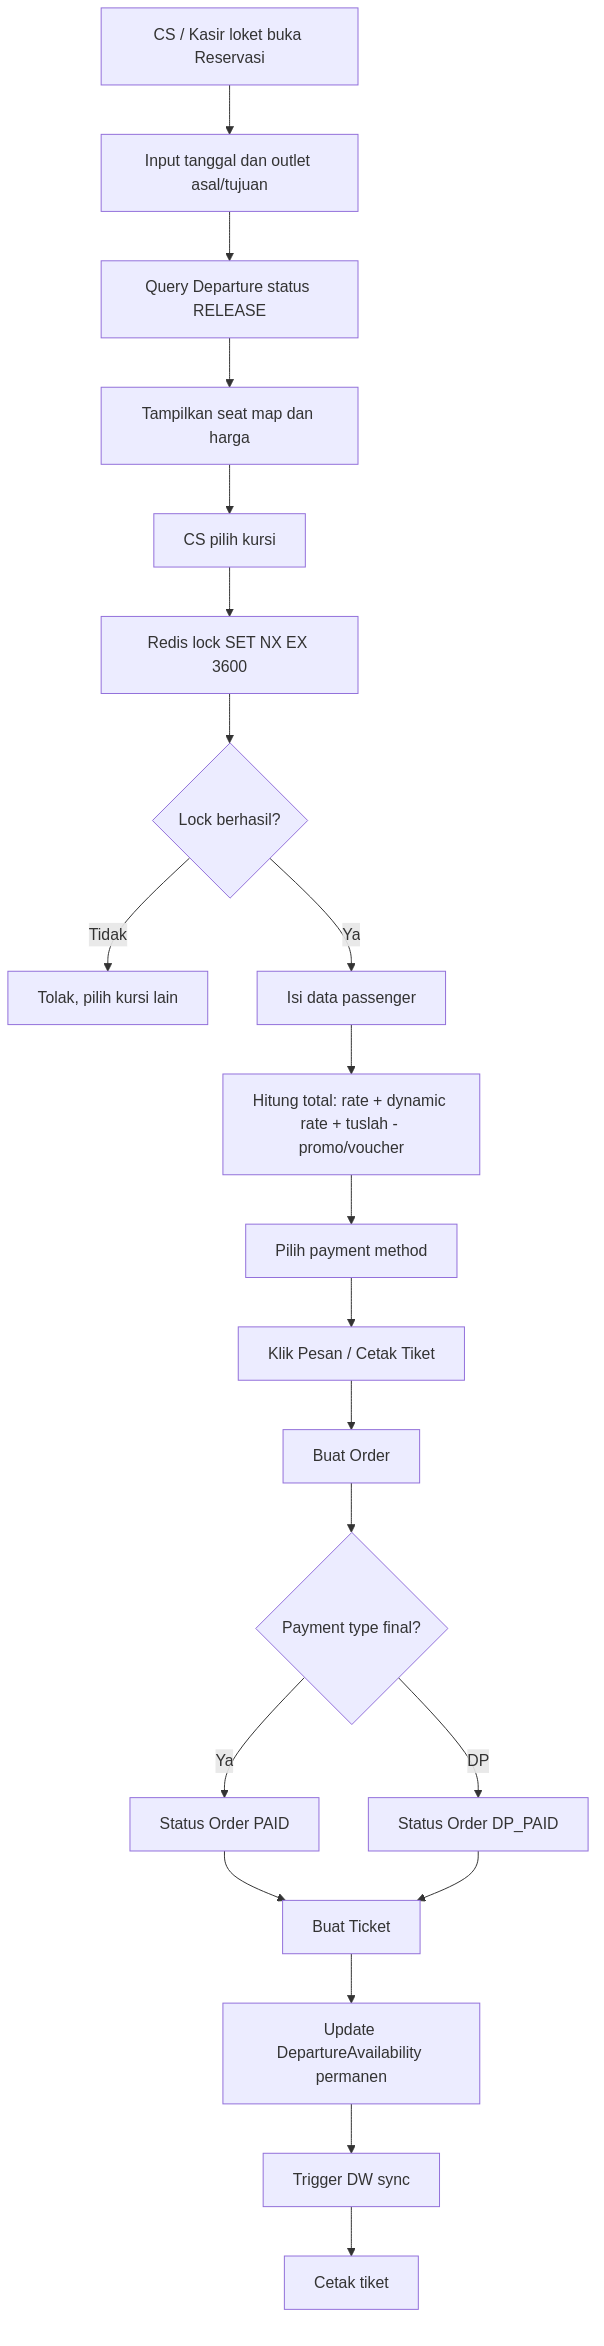
\includegraphics[width=\textwidth,height=0.85\textheight,keepaspectratio]{../booking_flow.png}
\end{figure}

\subsection{4.b OTA Booking Flow (API)}
\begin{figure}[H]
    \centering
    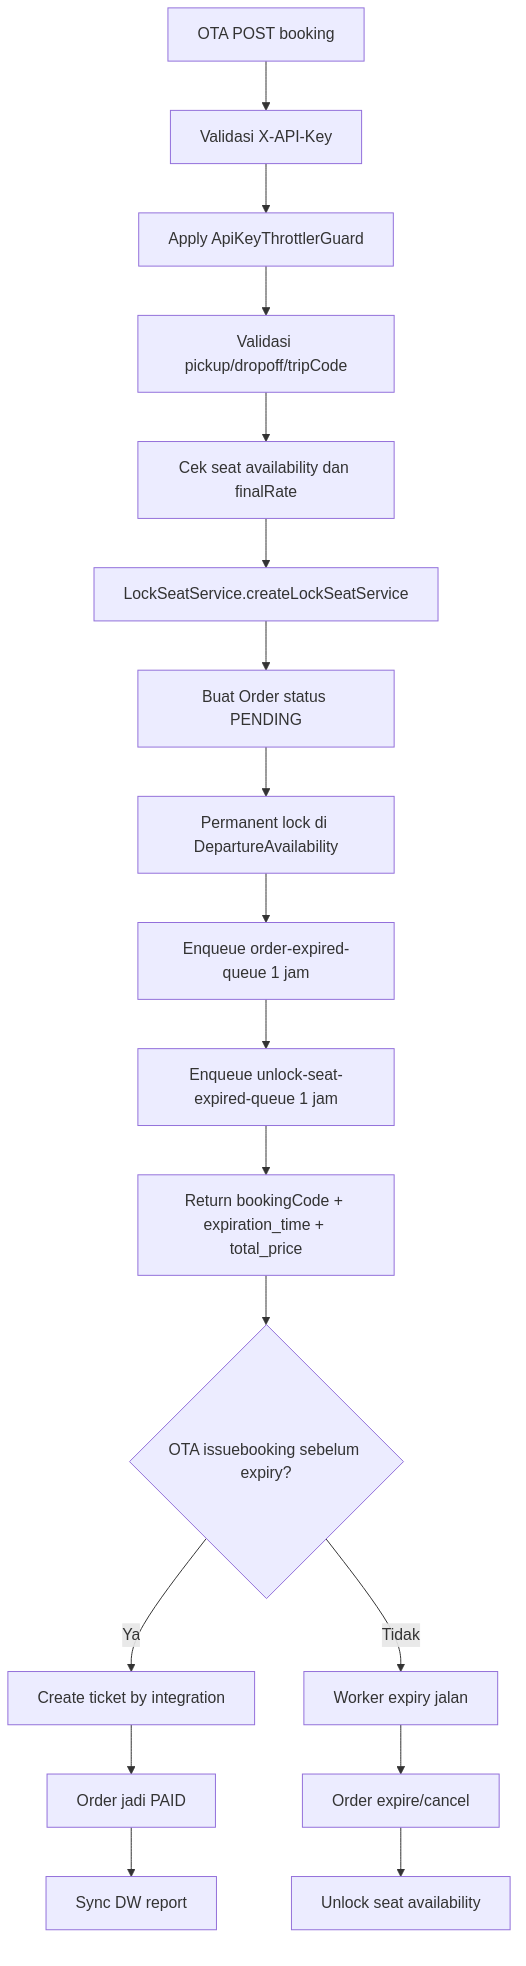
\includegraphics[width=\textwidth,height=0.85\textheight,keepaspectratio]{../ota_booking_flow.png}
\end{figure}

\subsection{4.c Finance Flow (Termasuk Overwrite, Manifest, \& Premi)}
\begin{figure}[H]
    \centering
    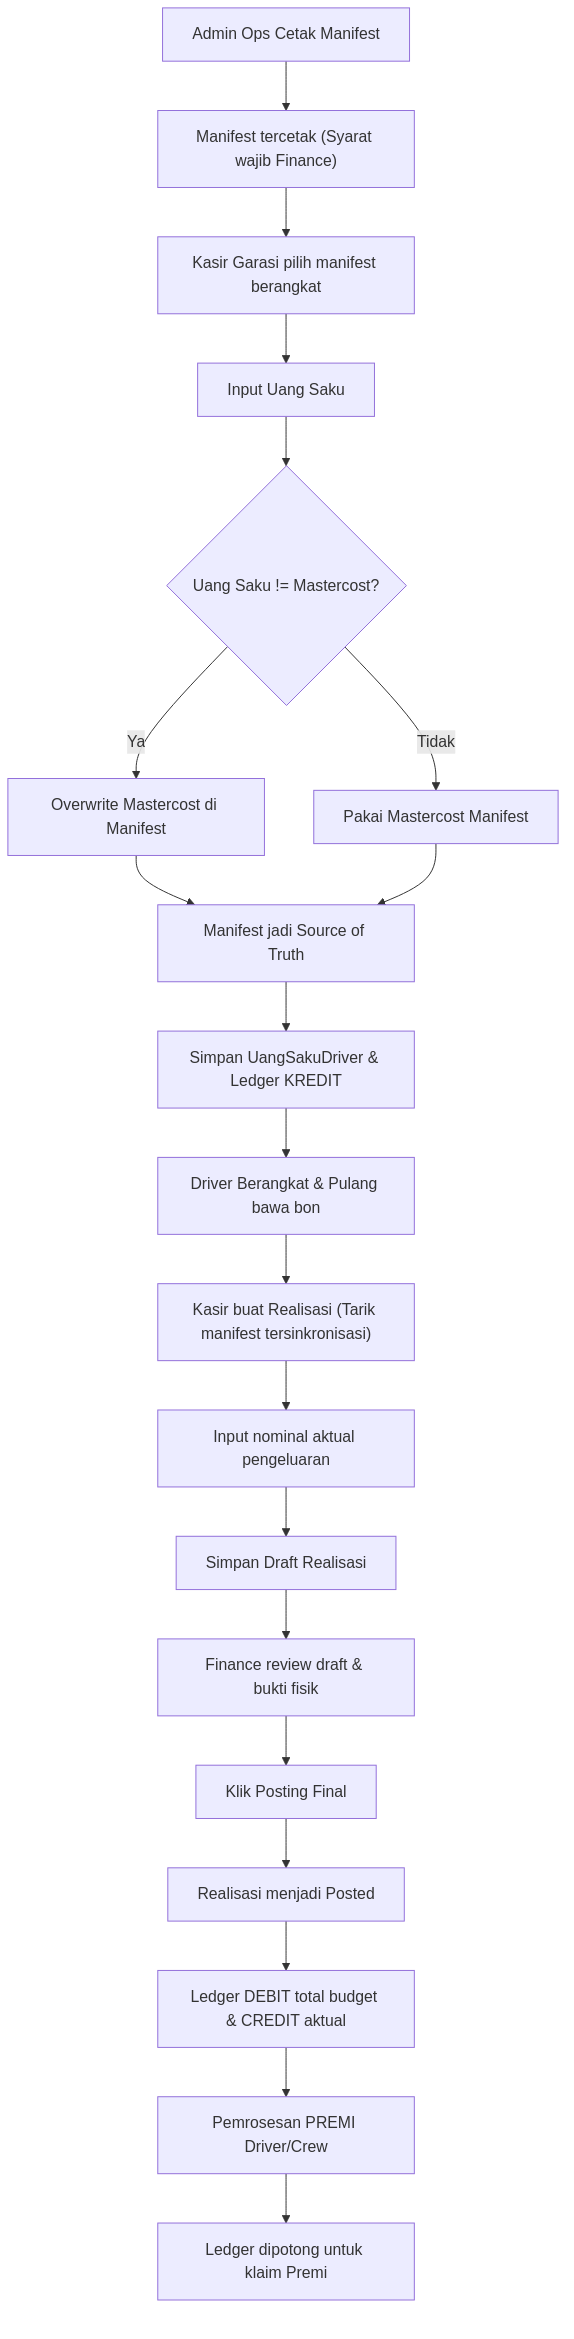
\includegraphics[width=\textwidth,height=0.85\textheight,keepaspectratio]{../finance_flow.png}
    \caption{Di sinilah Uang Saku meng-\\overwrite Manifest, Realisasi menarik manifest, Posting tereksekusi, dilanjut Premi.}
\end{figure}

\subsection{4.d Schedule Preparation Flow}
\begin{figure}[H]
    \centering
    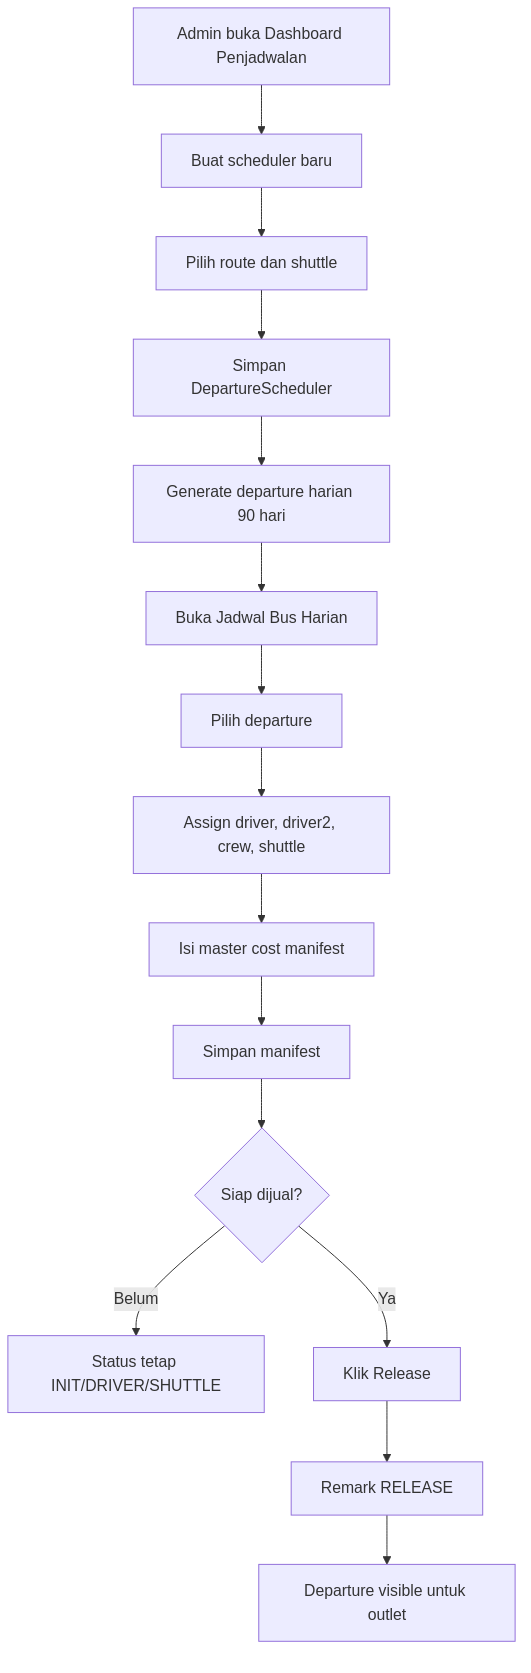
\includegraphics[width=\textwidth,height=0.85\textheight,keepaspectratio]{../schedule_flow.png}
\end{figure}

\subsection{4.e Seat Locking Race Condition Prevention}
\begin{figure}[H]
    \centering
    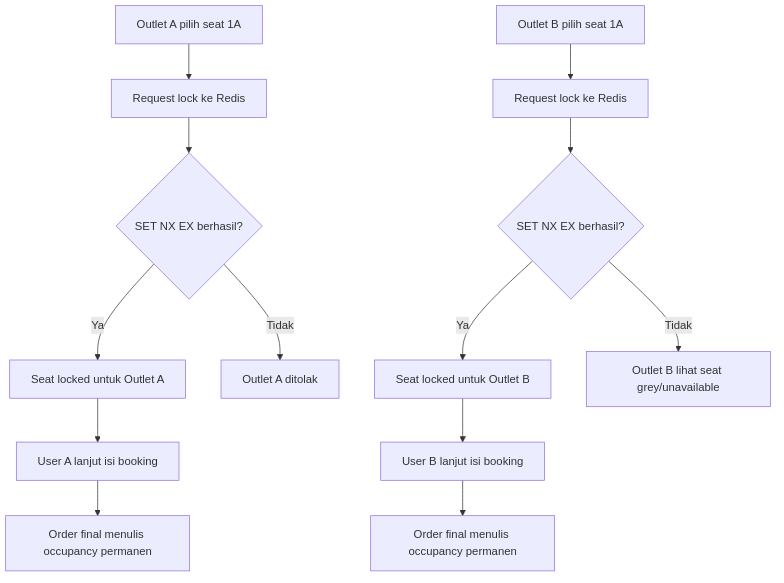
\includegraphics[width=\textwidth,height=0.85\textheight,keepaspectratio]{../race_condition_flow.png}
\end{figure}

\subsection{4.f Order Expiry BullMQ Worker Flow}
\begin{figure}[H]
    \centering
    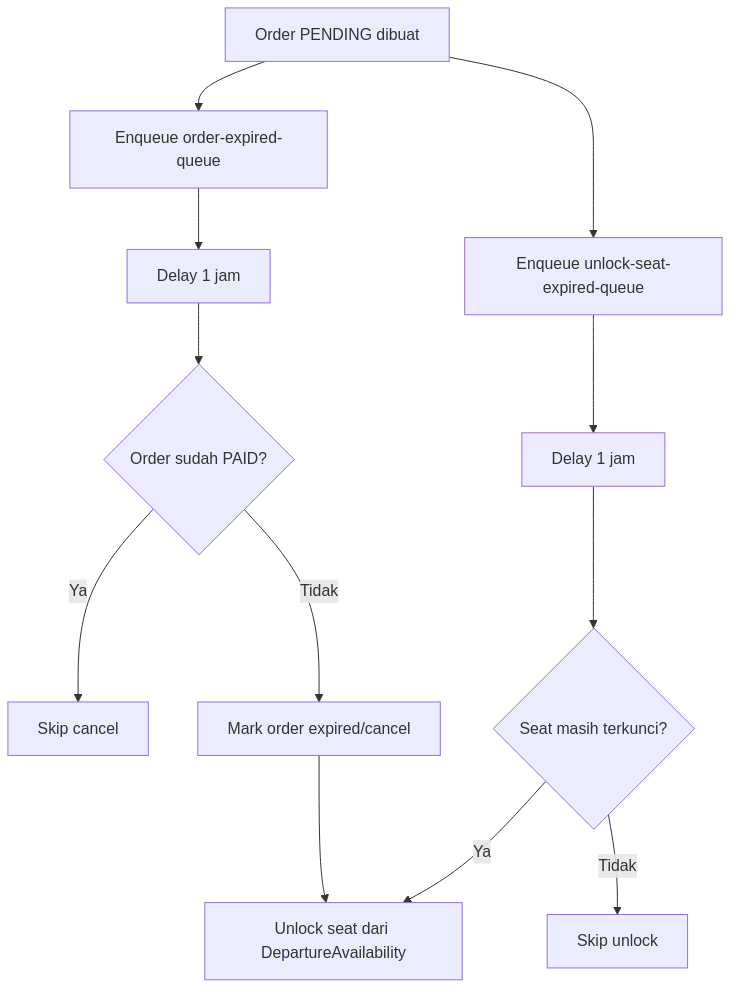
\includegraphics[width=\textwidth,height=0.85\textheight,keepaspectratio]{../expiry_flow.png}
\end{figure}

\clearpage
\section{5. Use Case Diagram \& Deskripsi}
\begin{figure}[H]
    \centering
    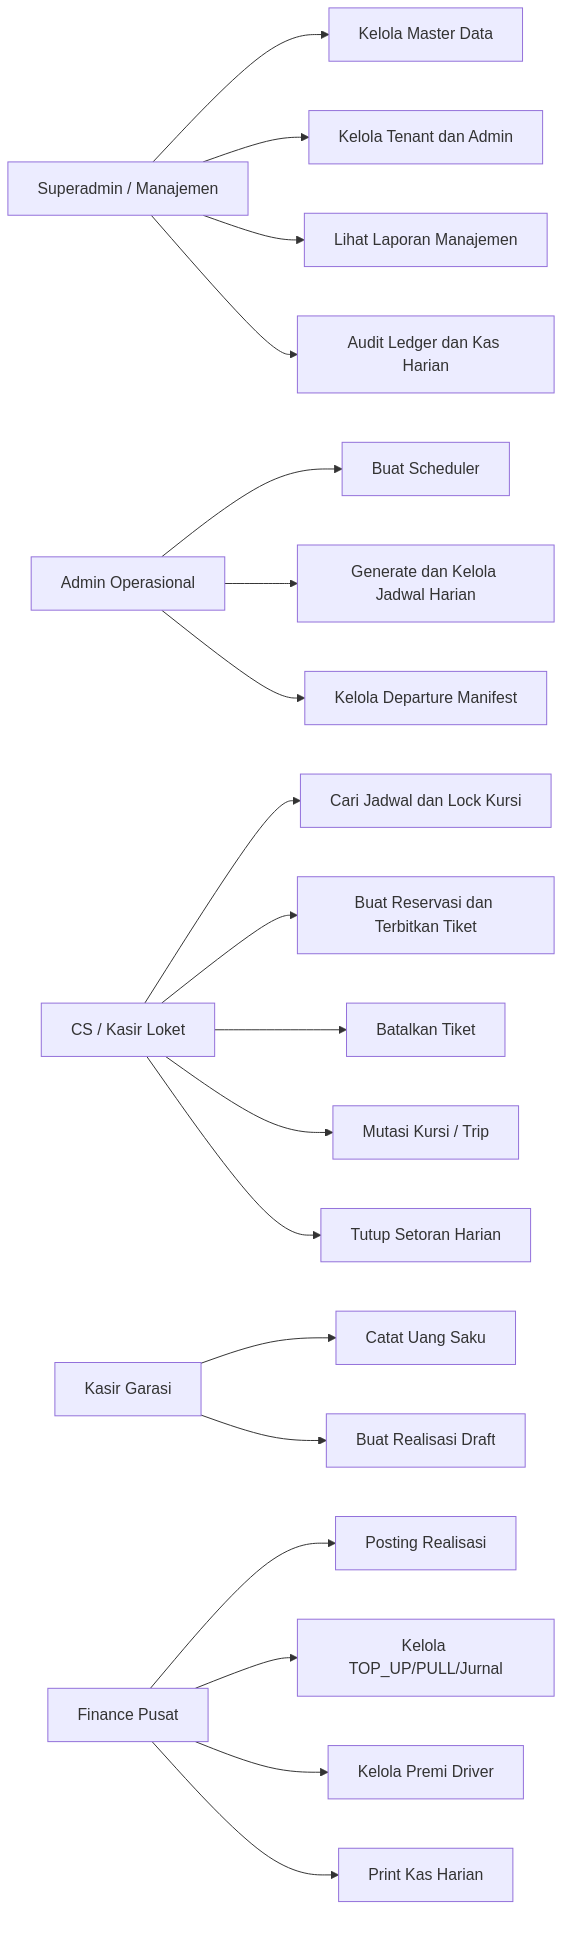
\includegraphics[width=\textwidth,height=0.85\textheight,keepaspectratio]{../usecase_diagram.png}
\end{figure}

\textbf{UC13: Catat Uang Saku (Overwriting logic)}
\begin{itemize}
    \item \textbf{Aktor}: Kasir Garasi
    \item \textbf{Prekondisi}: Manifest keberangkatan TELAH DICETAK dan dieksekusi Admin Operasional.
    \item \textbf{Skenario Utama}: Kasir memasukkan jumlah \textit{BBM, Tol}, bila berbeda dengan Mastercost asli di jadwal rutin, nilai ini OVERWRITE nominal di tabel manifest. Manifest dikunci menjadi \textit{Source of Truth}. Ledger Kredit tercatat.
\end{itemize}

\textbf{UC14: Buat Realisasi Draft}
\begin{itemize}
    \item \textbf{Aktor}: Kasir Garasi
    \item \textbf{Prekondisi}: Supir tiba membuahkan bon fisik.
    \item \textbf{Skenario Utama}: Kasir melengkapi rincian. \textbf{Acuan Realisasi sepenuhnya berasal dari Manifest yang sudah ter-overwrite dari Uang Saku tadi}. Draft diajukan ke Finance.
\end{itemize}

\textbf{UC17: Kelola Premi Driver/Crew (Baru Ditambahkan)}
\begin{itemize}
    \item \textbf{Aktor}: Finance Pusat
    \item \textbf{Prekondisi}: Supir berhasil merealisasikan perjalanannya.
    \item \textbf{Skenario Utama}: Finance memverifikasi daftar \textit{claim flag}. Rate dinilai berdasarkan role (Driver / Crew). Uang potongan ditarik dari Ledger. Status ditutup agar tidak diklaim dua kali.
\end{itemize}

\end{document}
